\subsection{Übung}
Gegenstand der Übung ist der nachfolgend abgebildete Immatrikulationsprozess.

\begin{figure}[h]
    \centering
    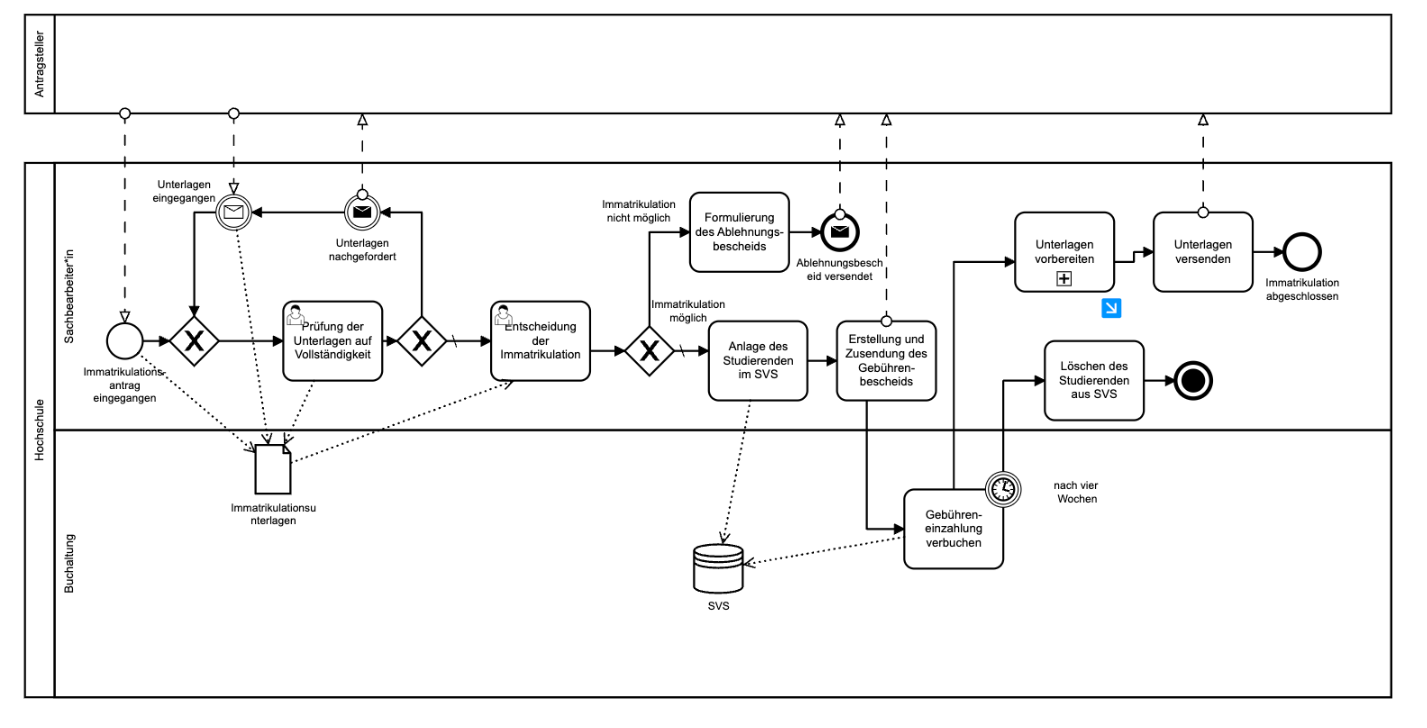
\includegraphics[width=\textwidth]{image/Uebung7.png}
    \caption{Übung 7}
    \label{fig:Uebung7}
\end{figure}

\subsubsection*{Aufgabe 7.1}
    \paragraph*{Aufgabe}
        Führen Sie eine Wertschöpfungsanalyse auf dem Immatrikulationsprozess durch. Zerlegen Sie dazu, wann immer es erforderlich ist, die Aktivitäten in einzelne Schritte. Kategorisieren Sie die Schritte in die in der Vorlesung vorgestellten Klassen:

        \begin{itemize}
            \item Wertschöpfend (WS)
            \item Geschäftswertschöpfend bzw. Geschäftsfördernd (GWS)
            \item Nicht-Wertschöpfend (NWS)
        \end{itemize}

        Begründen Sie jeweils die Zuordnung zu einer Kategorie!

    \paragraph*{Lösung}
        Keine Lösung

\subsubsection*{Aufgabe 7.2}
    \paragraph*{Aufgabe}
        Berechnen Sie die Durchlaufzeiteffizienz für den oben dargestellten Prozess, in dem Sie die folgenden Annahmen machen:

        \begin{itemize}
            \item In 10\% der Fälle sind die Unterlagen unvollständig
            \item In 25\% der Fälle werden Immatrikulationsanträge abgelehnt
            \item In 5\% der Fälle zahlen die Studierenden die Gebühren nicht innerhalb der vorgegebenen Frist
        \end{itemize}

        Darüber hinaus sind die durchschnittlichen Durchlaufzeiten bzw. die theoretischen Bearbeitungszeiten in der nachstehenden Tabelle zusammengefasst:

        \begin{tabular}{|>{\raggedright}p{5.5cm}|>{\raggedright}p{4cm}|>{\raggedright\arraybackslash}p{4cm}|}
            \hline
            \textbf{Aktivität} & \textbf{Durchschnittliche Durchlaufzeit} & \textbf{Theoretische Bearbeitungszeit} \\
            \hline
            Prüfung der Unterlagen auf Vollständigkeit & 15 Stunden & 1 Stunde \\
            \hline
            Entscheidung der Immatrikulation & 3 Stunden & 1 Stunde \\
            \hline
            Anlage des Studierenden im SVS & 4 Stunden & 0,25 Stunden \\
            \hline
            Erstellung und Zusendung des Gebührenbescheids & 1 Stunde & 0,5 Stunden \\
            \hline
            Gebühreneinzahlung verbuchen & 48 Stunden & 0,25 Stunden \\
            \hline
            Unterlagen vorbereiten & 12 Stunden & 0,5 Stunden \\
            \hline
            Unterlagen versenden & 2 Stunden & 0,25 Stunden \\
            \hline
            Löschen des Studierenden im SVS & 4 Stunden & 0,25 Stunden \\
            \hline
            Formulierung des Ablehnungsbescheids & 6 Stunden & 3 Stunden \\
            \hline
        \end{tabular}

        Beachten Sie, dass der Prozess eine externe Ausnahme enthält, durch die die durchschnittliche Durchlaufzeit erheblich gesteigert wird Typischerweise werden die durchschnittlichen Durchlaufzeiten nur für die regulären Prozessabläufe – also ohne die Berücksichtigung von Ausnahmen – berechnet. Berechnen Sie in dieser Übungsaufgabe aber die Durchlaufzeit mit Berücksichtigung der Ausnahme.

        Hinweis zur Lösung: Markieren und benennen Sie die einzelnen Bereiche des Diagramms, für die Sie die durchschnittlichen Durchlaufzeiten berechnen und führen Sie die Rechnungen in Teilrechnungen aus.
    \paragraph*{Lösung}
        \begin{itemize}
            \item DLZ: 
                \begin{itemize}
                    \item $\frac{15 Stunden}{1-0,1} = 16,7$
                    \item $16,7 + 3 + 0,25 * 6 + 0,75 * (4 + 1 + 48 + 0,95 * (12 + 2) + 0,05 * (672+4))$
                    \item $= 21,2 + 0,75*100,1$
                    \item $DLZ = 96,3 Stunden$
                \end{itemize}
            \item BAZ:
                \begin{itemize}
                    \item $\frac{1 Stunden}{1-0,1} = 1,1$
                    \item $1,1 + 1 + 0,25 * 3 + 0,75 * (0,25 + 0,5 + 0,25 + 0,95 * (0,5 + 0,25) + 0,05 * (672+0,25))$
                    \item $= 1,1 + 1 + 0,75 + 0,75 * 35,3$
                    \item $2,85 + 26,5$
                    \item $BAZ = 29,4$
                \end{itemize}
            \item BAZ: $DLE = \frac{29,4}{93,3}=0,32=32\%$
        \end{itemize}
        